\documentclass{ximera}

%\usepackage{todonotes}

\newcommand{\todo}{}

\usepackage{tkz-euclide}
\tikzset{>=stealth} %% cool arrow head
\tikzset{shorten <>/.style={ shorten >=#1, shorten <=#1 } } %% allows shorter vectors

\usepackage{tkz-tab}  %% sign charts
\usetikzlibrary{decorations.pathreplacing} 

\usetikzlibrary{backgrounds} %% for boxes around graphs
\usetikzlibrary{shapes,positioning}  %% Clouds and stars
\usetikzlibrary{matrix} %% for matrix
\usepgfplotslibrary{polar} %% for polar plots
\usetkzobj{all}
\usepackage[makeroom]{cancel} %% for strike outs
%\usepackage{mathtools} %% for pretty underbrace % Breaks Ximera
\usepackage{multicol}

\usepackage{polynom}



\usepackage[many]{tcolorbox}  %% for titled boxes
\newtcolorbox{xbox}[1]{%
    tikznode boxed title,
    enhanced,
    arc=0mm,
    interior style={white},
    attach boxed title to top center= {yshift=-\tcboxedtitleheight/2},
    fonttitle=\bfseries,
    colbacktitle=white,coltitle=black,
    boxed title style={size=normal,colframe=white,boxrule=0pt},
    title={#1}}


\usepackage{array}
\setlength{\extrarowheight}{+.1cm}   
\newdimen\digitwidth
\settowidth\digitwidth{9}
\def\divrule#1#2{
\noalign{\moveright#1\digitwidth
\vbox{\hrule width#2\digitwidth}}}





\newcommand{\RR}{\mathbb R}
\newcommand{\R}{\mathbb R}
\newcommand{\N}{\mathbb N}
\newcommand{\Z}{\mathbb Z}

%\renewcommand{\d}{\,d\!}
\renewcommand{\d}{\mathop{}\!d}
\newcommand{\dd}[2][]{\frac{\d #1}{\d #2}}
\newcommand{\pp}[2][]{\frac{\partial #1}{\partial #2}}
\renewcommand{\l}{\ell}
\newcommand{\ddx}{\frac{d}{\d x}}
\newcommand{\ddt}{\frac{d}{\d t}}

\newcommand{\zeroOverZero}{\ensuremath{\boldsymbol{\tfrac{0}{0}}}}
\newcommand{\inftyOverInfty}{\ensuremath{\boldsymbol{\tfrac{\infty}{\infty}}}}
\newcommand{\zeroOverInfty}{\ensuremath{\boldsymbol{\tfrac{0}{\infty}}}}
\newcommand{\zeroTimesInfty}{\ensuremath{\small\boldsymbol{0\cdot \infty}}}
\newcommand{\inftyMinusInfty}{\ensuremath{\small\boldsymbol{\infty - \infty}}}
\newcommand{\oneToInfty}{\ensuremath{\boldsymbol{1^\infty}}}
\newcommand{\zeroToZero}{\ensuremath{\boldsymbol{0^0}}}
\newcommand{\inftyToZero}{\ensuremath{\boldsymbol{\infty^0}}}



\newcommand{\numOverZero}{\ensuremath{\boldsymbol{\tfrac{\#}{0}}}}
\newcommand{\dfn}{\textbf}
%\newcommand{\unit}{\,\mathrm}
\newcommand{\unit}{\mathop{}\!\mathrm}
\newcommand{\eval}[1]{\bigg[ #1 \bigg]}
\newcommand{\seq}[1]{\left( #1 \right)}
\renewcommand{\epsilon}{\varepsilon}
\renewcommand{\iff}{\Leftrightarrow}

\DeclareMathOperator{\arccot}{arccot}
\DeclareMathOperator{\arcsec}{arcsec}
\DeclareMathOperator{\arccsc}{arccsc}
\DeclareMathOperator{\si}{Si}
\DeclareMathOperator{\proj}{proj}
\DeclareMathOperator{\scal}{scal}


\newcommand{\tightoverset}[2]{% for arrow vec
  \mathop{#2}\limits^{\vbox to -.5ex{\kern-0.75ex\hbox{$#1$}\vss}}}
\newcommand{\arrowvec}[1]{\tightoverset{\scriptstyle\rightharpoonup}{#1}}
\renewcommand{\vec}{\mathbf}
\newcommand{\veci}{\vec{i}}
\newcommand{\vecj}{\vec{j}}
\newcommand{\veck}{\vec{k}}
\newcommand{\vecl}{\boldsymbol{\l}}

\newcommand{\dotp}{\bullet}
\newcommand{\cross}{\boldsymbol\times}
\newcommand{\grad}{\boldsymbol\nabla}
\newcommand{\divergence}{\grad\dotp}
\newcommand{\curl}{\grad\cross}
%\DeclareMathOperator{\divergence}{divergence}
%\DeclareMathOperator{\curl}[1]{\grad\cross #1}


\colorlet{textColor}{black} 
\colorlet{background}{white}
\colorlet{penColor}{blue!50!black} % Color of a curve in a plot
\colorlet{penColor2}{red!50!black}% Color of a curve in a plot
\colorlet{penColor3}{red!50!blue} % Color of a curve in a plot
\colorlet{penColor4}{green!50!black} % Color of a curve in a plot
\colorlet{penColor5}{orange!80!black} % Color of a curve in a plot
\colorlet{fill1}{penColor!20} % Color of fill in a plot
\colorlet{fill2}{penColor2!20} % Color of fill in a plot
\colorlet{fillp}{fill1} % Color of positive area
\colorlet{filln}{penColor2!20} % Color of negative area
\colorlet{fill3}{penColor3!20} % Fill
\colorlet{fill4}{penColor4!20} % Fill
\colorlet{fill5}{penColor5!20} % Fill
\colorlet{gridColor}{gray!50} % Color of grid in a plot

\newcommand{\surfaceColor}{violet}
\newcommand{\surfaceColorTwo}{redyellow}
\newcommand{\sliceColor}{greenyellow}




\pgfmathdeclarefunction{gauss}{2}{% gives gaussian
  \pgfmathparse{1/(#2*sqrt(2*pi))*exp(-((x-#1)^2)/(2*#2^2))}%
}


%%%%%%%%%%%%%
%% Vectors
%%%%%%%%%%%%%

%% Simple horiz vectors
\renewcommand{\vector}[1]{\left\langle #1\right\rangle}


%% %% Complex Horiz Vectors with angle brackets
%% \makeatletter
%% \renewcommand{\vector}[2][ , ]{\left\langle%
%%   \def\nextitem{\def\nextitem{#1}}%
%%   \@for \el:=#2\do{\nextitem\el}\right\rangle%
%% }
%% \makeatother

%% %% Vertical Vectors
%% \def\vector#1{\begin{bmatrix}\vecListA#1,,\end{bmatrix}}
%% \def\vecListA#1,{\if,#1,\else #1\cr \expandafter \vecListA \fi}

%%%%%%%%%%%%%
%% End of vectors
%%%%%%%%%%%%%

%\newcommand{\fullwidth}{}
%\newcommand{\normalwidth}{}



%% makes a snazzy t-chart for evaluating functions
%\newenvironment{tchart}{\rowcolors{2}{}{background!90!textColor}\array}{\endarray}

%%This is to help with formatting on future title pages.
\newenvironment{sectionOutcomes}{}{} 



%% Flowchart stuff
%\tikzstyle{startstop} = [rectangle, rounded corners, minimum width=3cm, minimum height=1cm,text centered, draw=black]
%\tikzstyle{question} = [rectangle, minimum width=3cm, minimum height=1cm, text centered, draw=black]
%\tikzstyle{decision} = [trapezium, trapezium left angle=70, trapezium right angle=110, minimum width=3cm, minimum height=1cm, text centered, draw=black]
%\tikzstyle{question} = [rectangle, rounded corners, minimum width=3cm, minimum height=1cm,text centered, draw=black]
%\tikzstyle{process} = [rectangle, minimum width=3cm, minimum height=1cm, text centered, draw=black]
%\tikzstyle{decision} = [trapezium, trapezium left angle=70, trapezium right angle=110, minimum width=3cm, minimum height=1cm, text centered, draw=black]


\outcome{Know the graphs and properties of ``famous'' functions.}

\title[Dig-In:]{Graphs of polynomial functions}


\begin{document}
\begin{abstract}
  Polynomials are some of our favorite functions. 
\end{abstract}
\maketitle


\section{What do the graphs look like?}
We understand the graphs of polynomials of degrees $1$ and $2$ very well.

Polynomial functions with degree $1$ are referred to as linear polynomials.  This is due to the fact
that such a function can be written as $f(x) = mx + b$.  The graph of such a function is a straight line
with slope $m$ and $y$-intercept at $(0,b)$.

Quadratic functions, written as $f(x) = ax^2 + bx + c$ with $a \ne 0$, have parabolas as their graphs.
\begin{example}
	Sketch the graph of the function $f(x) = \frac{1}{2} x^2 + 2x + 1$.
	\begin{explanation}
		To plot the parabola, we first complete the square to write our function in the form $f(x) = a(x-h)^2 +k$.
		\begin{align*}
			f(x) &= \frac{1}{2} x^2 + 2x + 1 \\
				&= \frac{1}{2} \left( x^2+ 4x \right) + 1\\
				&= \frac{1}{2}\left( x^2 + 4x + 4\right) + 1 - \frac{1}{2} \cdot 4\\
				&= \frac{1}{2} \left( x+2 \right)^2 -1
		\end{align*} 
		The parabola we are looking for has vertex at $(-2, -1)$, opens upward (since $1/2 > 0$), and is wider than the standard
		$y=x^2$ parabola.
		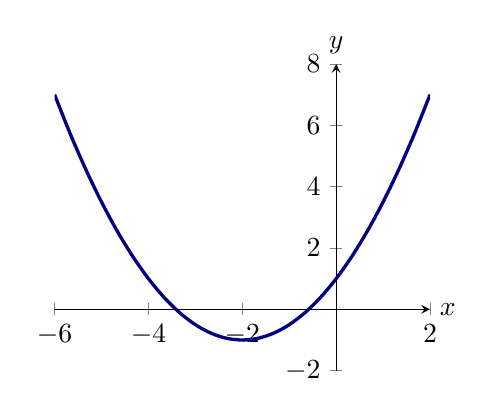
\begin{tikzpicture}
        			\begin{axis}[
          			domain=-6:2,
          			xmin=-6, xmax=2,
          			ymin=-2, ymax=8,
          			width=2.5in,
          			axis lines =middle, xlabel=$x$, ylabel=$y$,
          			every axis y label/.style={at=(current axis.above origin),anchor=south},
          			every axis x label/.style={at=(current axis.right of origin),anchor=west},
          			]
	 	 		\addplot [very thick, penColor, smooth] {0.5*x^2+2*x+1};
        			\end{axis}
      		\end{tikzpicture}
		
		In terms of graph transformations, we can think of this as the graph of $g(x) = x^2$, which has been shifted horizontally $2$ units to the left,
		vertically compressed by a factor of $\frac{1}{2}$, then shifted vertically $1$ unit downward.
	\end{explanation}
\end{example}


\begin{problem}
	Use the graph of $f(x) = 2x^2 - 4x + 3$ to estimate the value of $\lim_{x\to 2} f(x)$.
	\[ \begin{prompt} 
		\lim_{x\to 2} f(x) = \answer{3} 
	\end{prompt}\]
\end{problem} 

For polynomials of higher degree, we will have to take everything else we have been talking about and put it together.  
We need to understand the zeroes of the polynomial and its end behavior.  The zeroes will correspond to $x$-intercepts, and the
end behavior will tell us what happens out past those intercepts.

One upshot of the Fundamental Theorem of Algebra (in terms of graphing) is that when we plot a
polynomial of degree $n$, its graph will cross the $x$-axis \emph{at most}
$n$ times.  Each crossing corresponds to a real root of that polynomial.  (Complex roots do not give crossings!)

\begin{example}
	Sketch a rough graph of the function $f(x) = 2(x-1)^2(x+2)$.

	\begin{explanation}
		We start with the end behavior of this function.  It is a degree $3$ polynomial with leading coefficient $2$, so
		\begin{align*}
			\text{As} \quad x \to \infty \, ,  \quad & f(x) \to \infty \\
			\text{As} \quad x \to -\infty \, , \quad & f(x) \to -\infty 
		\end{align*}
		We also see from the factorization that $x=1$ is a zero of multiplicity $2$, and $x=-2$ is a zero of multiplicity $1$.
		That means our graph will have $x$-intercepts at those locations.
		
		At these $x$-intercepts, will the graph pass through the $x$-axis like a line does, or will it touch the axis and turn back
		around, like a parabola does at it's vertex?  To answer this, look at a sign-chart for $f$.

		\begin{center}
		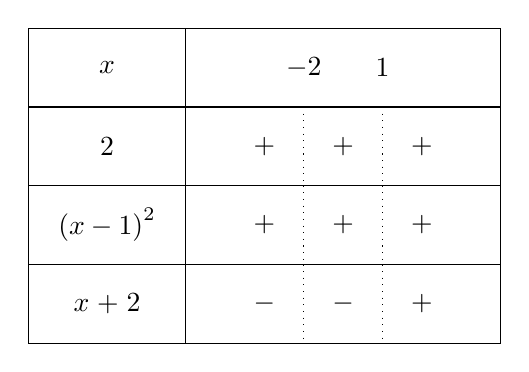
\begin{tikzpicture} 
			\tkzTabInit[lgt=2,espcl=1] 
				{$x$         /1, 
				$2$   /1, 
				$\left(x-1\right)^2$  /1,
				$x+2$       /1}% 
				{  , $-2$ , $1$ ,  }% 
			\tkzTabLine{ , + , t , + , t , + , }
			\tkzTabLine{ , + , t , + , t , + ,}
			\tkzTabLine{ , - , t , - , t , + ,  }
		\end{tikzpicture} 
		\end{center}
		
		Notice that around $x=-2$, only the $x+2$ factor changes signs.  That means $f(x)$ will change signs, so the graph will pass through the $x$-axis at $x=-2$.
		At $x=1$, however, the $(x-1)^2$ factor does NOT change signs (due to the even exponent).  That means $f(x)$ will turn around at that $x$-intercept.  Putting
		this together, we have the following graph.
		
		\begin{center}
		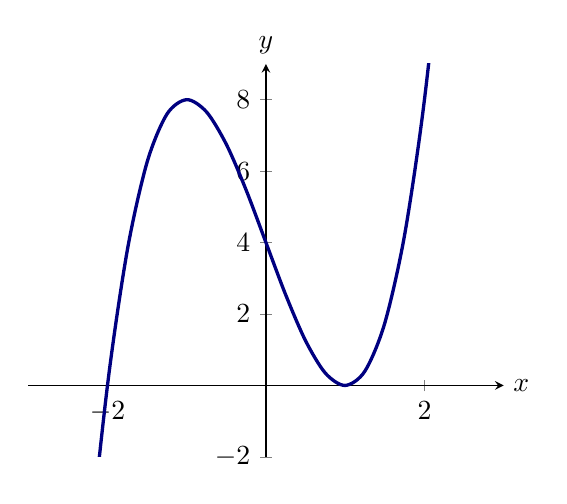
\begin{tikzpicture}
        			\begin{axis}[
          			domain=-3:3,
          			xmin=-3, xmax=3,
          			ymin=-2, ymax=9,
          			width=3in,
          			axis lines =middle, xlabel=$x$, ylabel=$y$,
          			every axis y label/.style={at=(current axis.above origin),anchor=south},
          			every axis x label/.style={at=(current axis.right of origin),anchor=west},
          			]
	 	 		\addplot [very thick, penColor, smooth] {2*((x-1)^2)*(x+2)};
        			\end{axis}
      		\end{tikzpicture}
		\end{center}
	\end{explanation}
\end{example}

\begin{problem}
	The function $f(x) = -4x^4 - 24x^3-32x^2+24x+36$ has zeroes at $x=-3$, $x=1$, and $x=-1$.
	At which of those $x$-intercepts does the graph of the function PASS THROUGH the $x$-axis?  (Don't use a graphing calculator)
	
	\begin{selectAll}
		\choice{At $x=-3$.}
		\choice[correct]{At $x=1$.}
		\choice[correct]{At $x=-1$.}
		\choice{At none of them.}
	\end{selectAll}
\end{problem}
Our discussion in that example showed that, given an $x$-intercept, we can determine if the graph passes through the $x$-axis or just turns around there, by
examining the multiplicity of that zero.  
\begin{theorem}
	Suppose the polynomial function $f$ has a zero at $x=a$ of multiplicity $n$.  If $n$ is odd, then the graph of $f$ will pass through $x$-axis at the point $(a,0)$.
	If $n$ is odd, then the graph of $f$ will intersect the $x$-axis at the point $(a,0)$, but not pass through the $x$-axis.
	
	More specifically: The graph of $f$ will resemble, at least locally near the point $(a,0)$, of the graph of $\pm (x-a)^n$.
\end{theorem}
This last statement means that if $x=4$ is a zero of $f$ with multiplicity $3$, then the graph of $f$ will pass through the $x$-axis at $(4,0)$, but it will flatten out the same
way that the graph of $y=x^3$ flattens out around the origin.

\begin{example}
  Here we see the the graphs of four polynomial functions.
  \begin{image}
    \begin{tabular}{cc}
      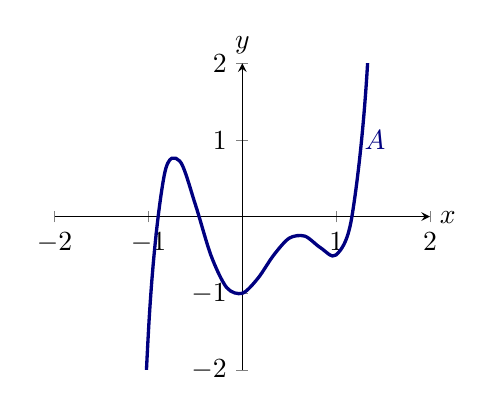
\begin{tikzpicture}
        \begin{axis}[
          domain=-2:2,
          xmin=-2, xmax=2,
          ymin=-2, ymax=2,
          width=2.5in,
          axis lines =middle, xlabel=$x$, ylabel=$y$,
          every axis y label/.style={at=(current axis.above origin),anchor=south},
          every axis x label/.style={at=(current axis.right of origin),anchor=west},
          ]
	  \addplot [very thick, penColor, smooth] {5*x^5-5*x^4-5*x^3+5*x^2+.5*x -1};
          \node at (axis cs:1.2, 1 ) [penColor,anchor=west] {$A$};
        \end{axis}
      \end{tikzpicture}
      &
      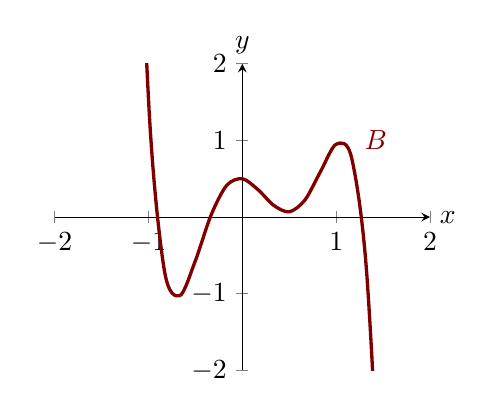
\begin{tikzpicture}
        \begin{axis}[
          domain=-2:2,
          xmin=-2, xmax=2,
          ymin=-2, ymax=2,
          width=2.5in,
          axis lines =middle, xlabel=$x$, ylabel=$y$,
          every axis y label/.style={at=(current axis.above origin),anchor=south},
          every axis x label/.style={at=(current axis.right of origin),anchor=west},
          ]
	  \addplot [very thick, penColor2, smooth] {-5*x^5+5*x^4+5*x^3-4.25*x^2-.3*x +.5};
          \node at (axis cs:1.2, 1 ) [penColor2,anchor=west] {$B$};
        \end{axis}
      \end{tikzpicture}\\
      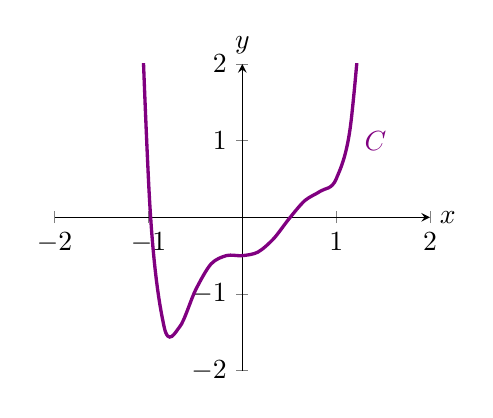
\begin{tikzpicture}
        \begin{axis}[
          domain=-2:2,
          xmin=-2, xmax=2,
          ymin=-2, ymax=2,
          width=2.5in,
          axis lines =middle, xlabel=$x$, ylabel=$y$,
          every axis y label/.style={at=(current axis.above origin),anchor=south},
          every axis x label/.style={at=(current axis.right of origin),anchor=west},
          ]
	  \addplot [very thick, penColor3, smooth] {5*x^6-5*x^5-5*x^4+5*x^3+x^2 -.5};
          \node at (axis cs:1.2, 1 ) [penColor3,anchor=west] {$C$};
        \end{axis}
      \end{tikzpicture}
      &
      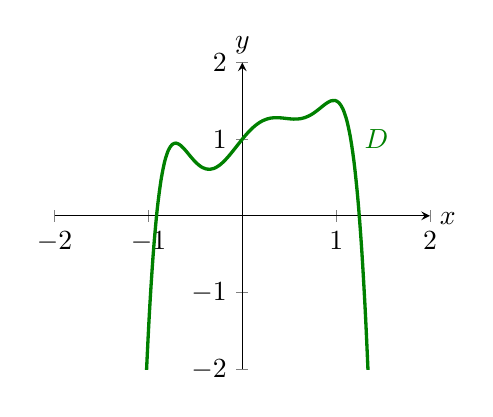
\begin{tikzpicture}
        \begin{axis}[
          domain=-2:2,
          xmin=-2, xmax=2,
          ymin=-2, ymax=2,
          width=2.5in,
          axis lines =middle, xlabel=$x$, ylabel=$y$,
          every axis y label/.style={at=(current axis.above origin),anchor=south},
          every axis x label/.style={at=(current axis.right of origin),anchor=west},
          ]
	  \addplot [very thick, penColor4, smooth,samples=100] {-5*x^6+5*x^5+5*x^4-5*x^3-x^2+1.5*x+1};
          \node at (axis cs:1.2, 1 ) [penColor4,anchor=west] {$D$};
        \end{axis}
      \end{tikzpicture}
    \end{tabular}
  \end{image}
  For each of the curves, determine if the polynomial has
  \textbf{even} or \textbf{odd} degree, and if the leading coefficient
  (the one next to the highest power of $x$) of the polynomial is
  \textbf{positive} or \textbf{negative}.
  \begin{explanation}\hfil
    \begin{itemize}
    \item Curve $A$ is defined by an
      \wordChoice{\choice{even}\choice[correct]{odd}} degree
      polynomial with a \wordChoice{\choice[correct]{positive}\choice{negative}}
      leading term.
    \item Curve $B$ is defined by an
      \wordChoice{\choice{even}\choice[correct]{odd}} degree
      polynomial with a
      \wordChoice{\choice{positive}\choice[correct]{negative}} leading
      term.
    \item Curve $C$ is defined by an
      \wordChoice{\choice[correct]{even}\choice{odd}} degree
      polynomial with a \wordChoice{\choice[correct]{positive}\choice{negative}}
      leading term.
    \item Curve $D$ is defined by an
      \wordChoice{\choice[correct]{even}\choice{odd}} degree
      polynomial with a \wordChoice{\choice{positive}\choice[correct]{negative}}
      leading term.
    \end{itemize}
  \end{explanation}
\end{example}


\end{document}
